
\begin{figure}[t]
  \centering
  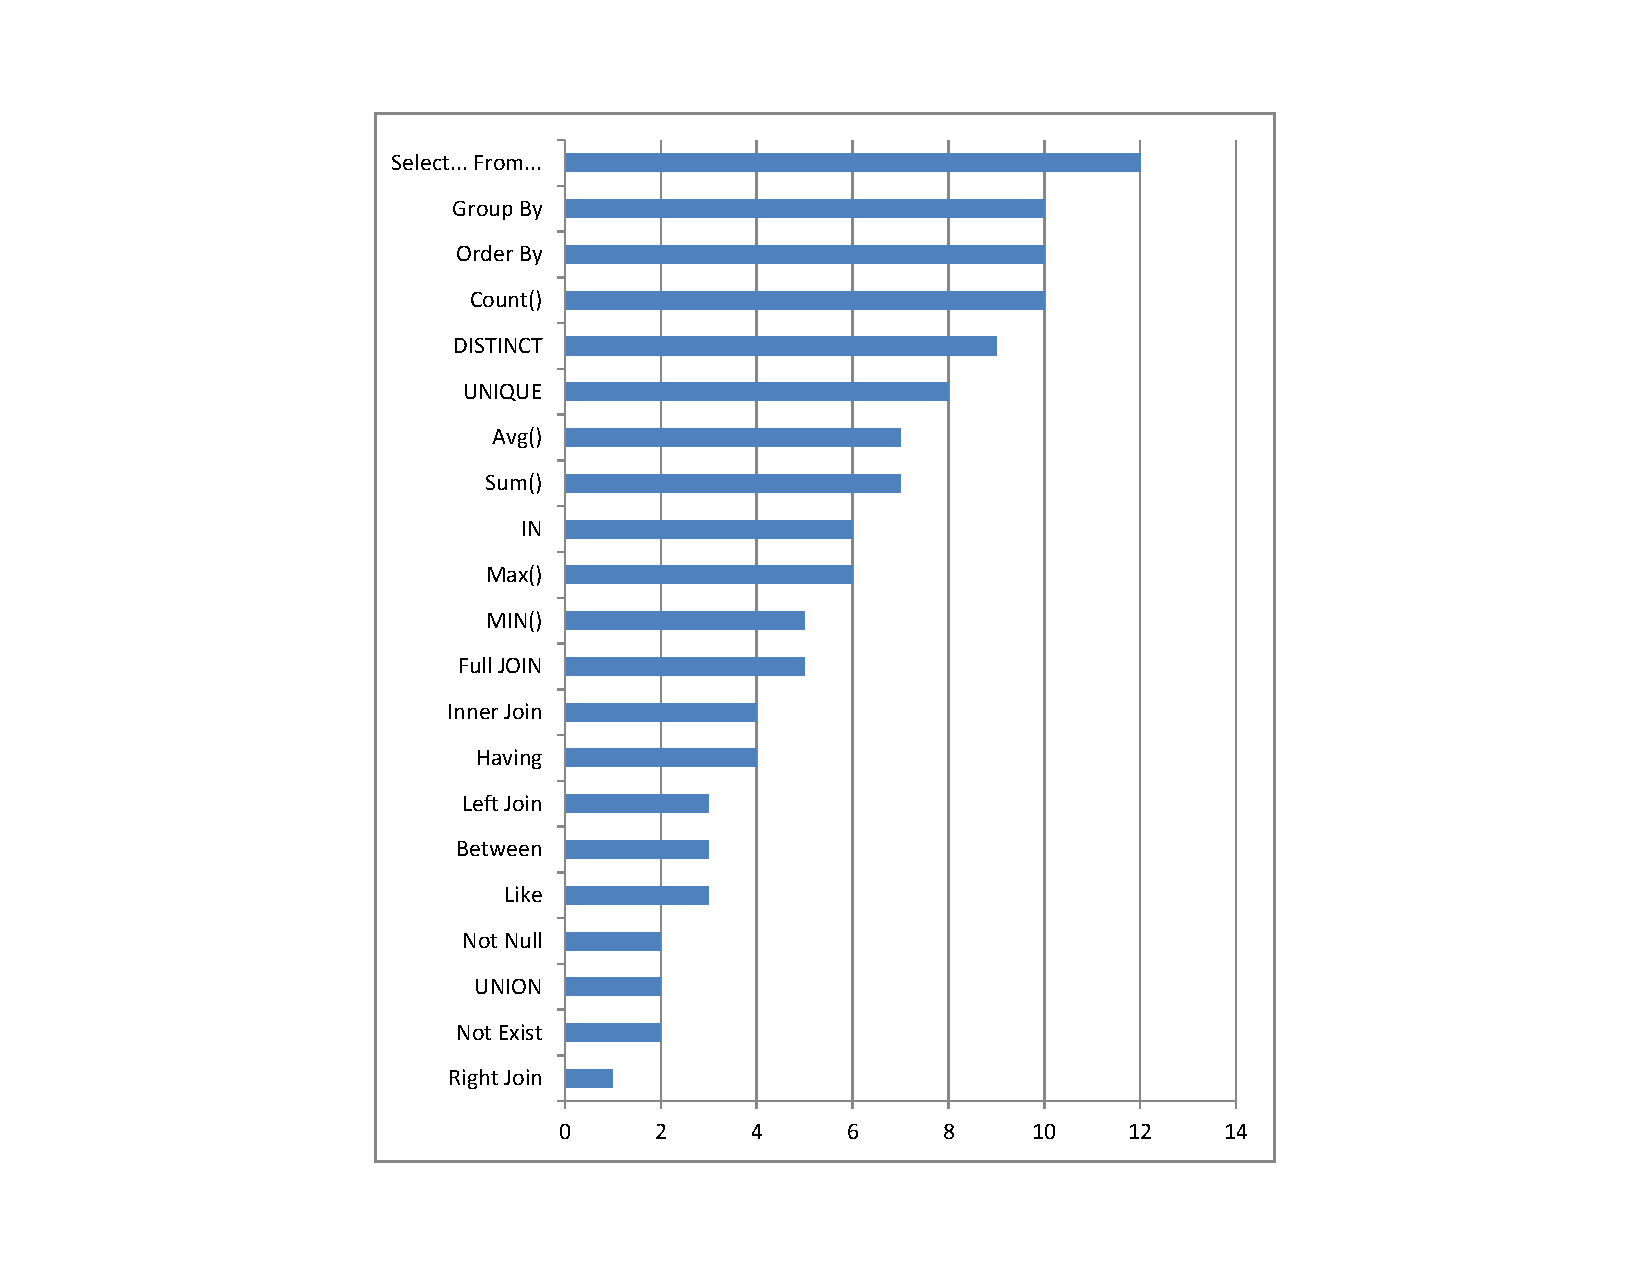
\includegraphics[scale=0.50]{survey}
  \vspace*{-1.0ex}\caption {{\label{fig:survey} Survey results...
}}

\end{figure}

\newcommand{\q}{\langle query\rangle}
\newcommand{\db}{\langle db\rangle}
\newcommand{\pat}{\langle pat\rangle}
\newcommand{\bug}{\langle bug\rangle}
\newcommand{\dist}{\langle distance\rangle}
\newcommand{\sem}[1]{\llbracket #1\rrbracket}
\newcommand{\lit}[1]{\texttt{#1}}

\newcommand{\column}{\langle column\rangle}
\newcommand{\dbtable}{\langle table\rangle}
\newcommand{\cond}{\langle cond\rangle}
\newcommand{\op}{\langle op\rangle}
\newcommand{\e}{\langle expr\rangle}
\newcommand{\ce}{\langle cexpr\rangle}

\begin{figure}[t]
%\scriptsize{%
\footnotesize%
\begin{align*}
\q ::= {} 
	& \texttt{ SELECT } \e^+ \texttt{ FROM } \dbtable^+ \\
        & \texttt{ WHERE } \cond^+ \\ 
	&  \texttt{ GROUP BY } \column^+ \texttt{ HAVING } \cond^+\\
	&  \texttt{ ORDER BY } \column^+ \\
\dbtable::= {} &\ atom \\
\column ::= {} &\ \dbtable.atom\\
\cond ::= {} &\ \ \cond \;\texttt{\&\&}\; \cond \\ 
    & |\ \cond \;\texttt{||}\; \cond \\
    & |\ \texttt{(}\;\cond\;\texttt{)} \\
    & |\ \ce \;\op\; \ce \\
    & |\ \texttt{NOT EXIST} \;(\q) \\
\op ::= {} &\ \ \texttt{=} \;\;|\;\; \texttt{>}  \;\;|\;\; \texttt{<}\\
\ce ::= {} &\ \ const \;\;|\;\; \column  \;\; \\
\e ::= {} & \ce \;\;|\ count(\column) \\
    & |\ sum(\column) \;\;|\ max(\column) \;\;|\ min(\column) 
\end{align*}
\normalsize%
\caption{Syntax of the supported SQL subset.}
\label{fig:syntax}
\end{figure}


\section{Supported SQL Subset}
\label{sec:langsubset}

This section presents the design of
a supported SQL subset in \ourtool.

The first step is to ... \todo{}
However, no systematic study has ever been conducted to this end, 
and little empirical knowledge has ever been provided. Without 
such study or empirical knowledge, understanding XXX
 remains difficult.

To address this issue, we conduct a online survey
and a series of follow-up email interviews.

\subsection{Online Survey: Eliciting Design Requirements}

\todo{Explain why a survey is needed (the langauge is
too big). It will become intractable. And how}

Decide the important
\todo{Took a different way than existing work in eliciting
design requirement.}

Our online survey consists of 6 questions that can be
divided into three parts. The first part includes
simple demographic questions about participants.
In the second part, participants were asked to select
their most-often \todo{most important?} used SQL language features. 
Instead of directly asking participants about the SQL
features, which might be vague and difficult to respond,
we presented them a list of \textit{all} standard
SQL features in writing a query.
Additionally, participants were asked to report their 
own experience in writing SQL queries in the third part of the survey.

Before distributing our survey, we conducted pilot
interviews with three graduate students with XXX experience
at University of Washington. We ran the survey with them and
made notes of their comments. According to their feedback,
we refined the survey questions and adjusted the wording to
make sure that the questions are relevant and clear.


We sent out invitation to graduate mailing lists at
University of Washington, and posted our survey on
professional online forums (e.g., StackOverflow).
As of April 2013, we received \respnum responses.
On average, the respondents have XXX years of experience
in Computer Science, and XXX years of experience in
using database.

Figure~\ref{}

\subsection{Syntax}


Figure~\ref{fig:syntax} defines the syntax of the supported language,
which is a subset of the standard SQL 93 language. This SQL subset
supports common query operations across multiple tables (i.e.,
\CodeIn{select} ... \CodeIn{from} ... \CodeIn{where}..), and 
conjunction of predicates. The language
subset shares the same semantics with the standard SQL language.

\todo{some design rationale}
1. discard some vendor-specific grammars, like top in Microsoft,

2 discard fuzzy matching part for example, like " ... ", wildcards,
makes undecidable, can use string manipulation.

3. exclude delete, update query statement, because we focus on query

4. Omit distinct, in (which can be replaced by NOT EXIST, or condition query)

5. omit between, discard Left Joint, Right Join, only remaining Full Join

6. Not Null (can be simply replaced by != NULL)

7. Nested query can always be re-written using conditions


\todo{revise the following}
Differing from language subsets used in the
existing work~\cite{DasSarma:2010}, our language subset
supporting
joining operations across multiple tables, and includes
widely-used database operations such as \CodeIn{group by},
\CodeIn{order by}, and \CodeIn{having}, as
well as a few common aggregation functions such as \CodeIn{count}, \CodeIn{sum},
\CodeIn{max}, and \CodeIn{min}.

%\todo{remove}
%As we will show in Section~\ref{sec:evaluation}, this
%subset, though far from completion, is expressive enough for answering
%many evaluated SQL exercises from a textbook and some real problems
%from online forums.

\subsection{Follow-up Interviews: Feedback about the SQL Subset}

After prototyping the SQL language in Figure~\ref{},
we performed follow-up email interviews to gain
participants' feedback about the tailored SQL
subset. Participants were first asked to rate
the expressiveness of the SQL subset in Figure~\ref{}
on a 6-point scale (5-sufficient; 0-not sufficient at all),
and then to provide their comments.
\todo{xxx}.

